% Options for packages loaded elsewhere
\PassOptionsToPackage{unicode}{hyperref}
\PassOptionsToPackage{hyphens}{url}
%
\documentclass[
]{article}
\usepackage{amsmath,amssymb}
\usepackage{lmodern}
\usepackage{iftex}
\ifPDFTeX
  \usepackage[T1]{fontenc}
  \usepackage[utf8]{inputenc}
  \usepackage{textcomp} % provide euro and other symbols
\else % if luatex or xetex
  \usepackage{unicode-math}
  \defaultfontfeatures{Scale=MatchLowercase}
  \defaultfontfeatures[\rmfamily]{Ligatures=TeX,Scale=1}
\fi
% Use upquote if available, for straight quotes in verbatim environments
\IfFileExists{upquote.sty}{\usepackage{upquote}}{}
\IfFileExists{microtype.sty}{% use microtype if available
  \usepackage[]{microtype}
  \UseMicrotypeSet[protrusion]{basicmath} % disable protrusion for tt fonts
}{}
\makeatletter
\@ifundefined{KOMAClassName}{% if non-KOMA class
  \IfFileExists{parskip.sty}{%
    \usepackage{parskip}
  }{% else
    \setlength{\parindent}{0pt}
    \setlength{\parskip}{6pt plus 2pt minus 1pt}}
}{% if KOMA class
  \KOMAoptions{parskip=half}}
\makeatother
\usepackage{xcolor}
\usepackage[margin=1in]{geometry}
\usepackage{graphicx}
\makeatletter
\def\maxwidth{\ifdim\Gin@nat@width>\linewidth\linewidth\else\Gin@nat@width\fi}
\def\maxheight{\ifdim\Gin@nat@height>\textheight\textheight\else\Gin@nat@height\fi}
\makeatother
% Scale images if necessary, so that they will not overflow the page
% margins by default, and it is still possible to overwrite the defaults
% using explicit options in \includegraphics[width, height, ...]{}
\setkeys{Gin}{width=\maxwidth,height=\maxheight,keepaspectratio}
% Set default figure placement to htbp
\makeatletter
\def\fps@figure{htbp}
\makeatother
\setlength{\emergencystretch}{3em} % prevent overfull lines
\providecommand{\tightlist}{%
  \setlength{\itemsep}{0pt}\setlength{\parskip}{0pt}}
\setcounter{secnumdepth}{-\maxdimen} % remove section numbering
\usepackage{bbm, amsmath}
\usepackage{booktabs}
\usepackage{longtable}
\usepackage{array}
\usepackage{multirow}
\usepackage{wrapfig}
\usepackage{float}
\usepackage{colortbl}
\usepackage{pdflscape}
\usepackage{tabu}
\usepackage{threeparttable}
\usepackage{threeparttablex}
\usepackage[normalem]{ulem}
\usepackage{makecell}
\usepackage{xcolor}
\ifLuaTeX
  \usepackage{selnolig}  % disable illegal ligatures
\fi
\IfFileExists{bookmark.sty}{\usepackage{bookmark}}{\usepackage{hyperref}}
\IfFileExists{xurl.sty}{\usepackage{xurl}}{} % add URL line breaks if available
\urlstyle{same} % disable monospaced font for URLs
\hypersetup{
  pdftitle={Report for PS 1},
  pdfauthor={Jack Xie; Rebecca Car; Kazi Jahurul Islam},
  hidelinks,
  pdfcreator={LaTeX via pandoc}}

\title{Report for PS 1}
\author{Jack Xie \and Rebecca Car \and Kazi Jahurul Islam}
\date{}

\begin{document}
\maketitle

\hypertarget{asset-return-predictability-and-market-efficiency}{%
\section{Asset Return Predictability and Market
Efficiency}\label{asset-return-predictability-and-market-efficiency}}

\hypertarget{testing-for-asset-return-predictability}{%
\subsection{Testing for asset return
predictability}\label{testing-for-asset-return-predictability}}

In this part of the report we are going to discuss the test for asset
return predictability based on autocorrelation functions, Ljung-Box
statistics and variance ratio tests using the \textbf{Dow Jones Daily}
and \textbf{Dow Jones Weekly} data set.

\hypertarget{daily-and-weekly-data}{%
\subsubsection{Daily and weekly data:}\label{daily-and-weekly-data}}

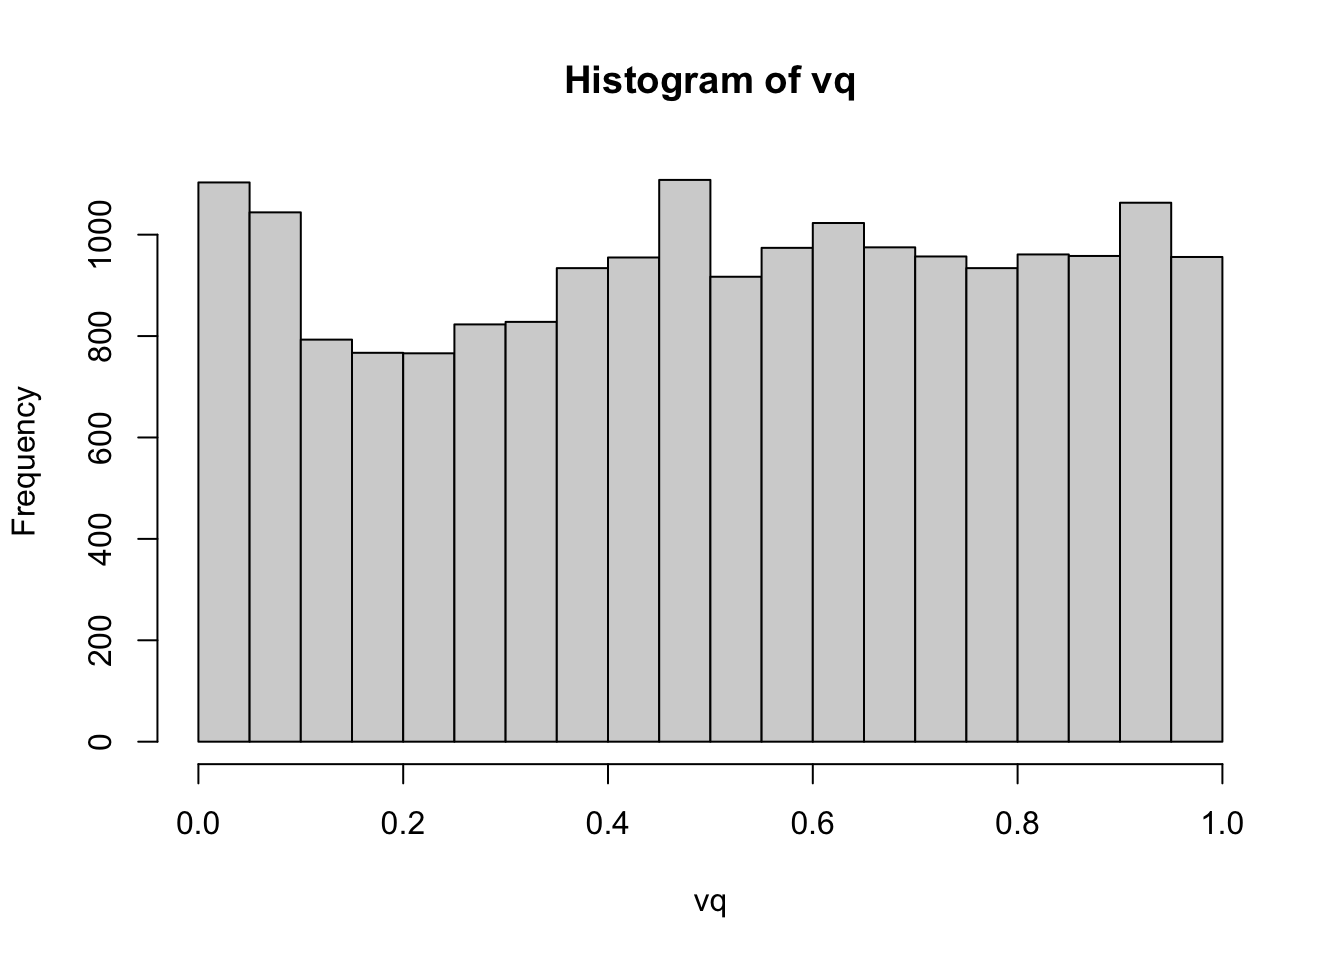
\includegraphics{PS1_Report_files/figure-latex/unnamed-chunk-1-1.pdf}

In the above figures we observe significant lags from the \textbf{ACF}
and \textbf{PACF} plot for both \textbf{Dow Jones Daily} and
\textbf{Dow Jones Weekly} data. Which is the indication of
autocorrealatios.

\newpage

Now at this point we are going to apply Lung-Box test to check
autocorrelation for both data set. The results are presented below:

\begin{table}

\caption{\label{tab:unnamed-chunk-3}This table presents p-values of Ljung-Box and variance ratio tests of no autocorrelation for daily and weekly data. Stars indicate significance levels. *: p-value < 0.1, **: p-value < 0.5, ***: p-value <0.01.}
\centering
\begin{tabular}[t]{l|l|l}
\hline
  & Test & P-value\\
\hline
5(DJ\_d) & 329.90 & 0***\\
\hline
10(DJ\_d) & 371.60 & 0***\\
\hline
20(DJ\_d) & 388.93 & 0***\\
\hline
5(DJ\_w) & 5.14 & 0.399\\
\hline
10(DJ\_w) & 13.59 & 0.192\\
\hline
20(DJ\_w) & 23.32 & 0.273\\
\hline
VR(DJ\_d) & 5.75 & 0.00***\\
\hline
VR(DJ\_w) & -0.20 & 0.84\\
\hline
\end{tabular}
\end{table}

We present the p-values of the Ljung-Box test for each index with
\(k \in \{5, 10, 20\}\) lags below, with degrees of freedom
\(d = k - 2\).

It is interesting to note that Ljunk-box with five and ten and twenty
lags and variance ratio statistics are highly significant for daily log
returns. On the other hand to daily returns, the respective
autocorrelation tests are insignificant for weekly log returns. So we
can be concluded that the daily returns are autocorrelated and weekly
returns may not be auto correlated.

\hypertarget{aggregated-data}{%
\subsubsection{Aggregated data:}\label{aggregated-data}}

\includegraphics{PS1_Report_files/figure-latex/unnamed-chunk-4-1.pdf}

From the above plots we observe for 2 day Dow Jones return, both acf and
pacf exibits some tailing off so they can be modeled with ARMA model,
there its a indication of autocorrelations. But for 2 week Dow Jones
return there are no significant tail off which indicates theres maybe no
auto correlation present in 2 weekly Dow Jones asset returns.

Now we are going to apply Lung-Box test to check autocorrelation for 2
day and 2 week data set. The results are presented below:

\begin{table}

\caption{\label{tab:unnamed-chunk-5}This table presents p-values of Ljung-Box and variance ratio tests of no autocorrelation for 2-day and 2-week Stars indicate significance levels. *: p-value < 0.1, **: p-value < 0.5, ***: p-value <0.01.}
\centering
\begin{tabular}[t]{l|l|l}
\hline
  & Test & P-value\\
\hline
5(DJ\_d) & 37.20 & 5.46e-07***\\
\hline
10(DJ\_d) & 57.03 & 1.32e-08***\\
\hline
20(DJ\_d) & 87.66 & 1.89e-10***\\
\hline
5(DJ\_w) & 4.43 & 0.489\\
\hline
10(DJ\_w) & 8.84 & 0.547\\
\hline
20(DJ\_w) & 21.54 & 0.366\\
\hline
VR(DJ\_d) & 0.45 & 0.65\\
\hline
VR(DJ\_w) & 0.48 & 0.63\\
\hline
\end{tabular}
\end{table}

We observe here that, Ljunk-box with five and ten and twenty lags
statistics are highly significant for 2-day log returns. On the other
hand to daily returns, the respective autocorrelation tests are
insignificant for 2-week log returns. Here we do notice that variance
ratio statistics are no significant for both 2-day and 2-week agrregated
data. So we can be concluded that the daily returns are autocorrelated
and weekly returns may not be autocorrelated.

\textbf{Note: need to interpret variance ratio statistics.}

Now we are going to look at 5 day and 10 day agrregated data in the form
of ACF and PACF plot.

\includegraphics{PS1_Report_files/figure-latex/unnamed-chunk-6-1.pdf}

From the above plots we observe for 5-day and 10-day Dow Jones return,
acf does not exibit any tailing off and pacf exibits some tailing off so
they can be modeled with MA model, there its a indication of
autocorrelations.

Now we are going to apply Lung-Box test to check autocorrelation for
5-day and 10-day data set. The results are presented below:

\begin{table}

\caption{\label{tab:unnamed-chunk-7}This table presents p-values of Ljung-Box and variance ratio tests of no autocorrelation for 5-day and 10-day Stars indicate significance levels. *: p-value < 0.1, **: p-value < 0.5, ***: p-value <0.01.}
\centering
\begin{tabular}[t]{l|l|l}
\hline
  & Test & P-value\\
\hline
5(DJ\_d) & 5.20 & 0.392\\
\hline
10(DJ\_d) & 12.39 & 0.26\\
\hline
20(DJ\_d) & 45.68 & 0.000893***\\
\hline
5(DJ\_d) & 3.38 & 0.642\\
\hline
10(DJ\_d) & 9.16 & 0.517\\
\hline
20(DJ\_d) & 35.16 & 0.0193**\\
\hline
VR(DJ\_d) & 1.65 & 0.10\\
\hline
VR(DJ\_w) & 0.89 & 0.37\\
\hline
\end{tabular}
\end{table}

We observe here that, Ljunk-box with five, ten lags and variance ratio
statistics are non significant for 5-day and 10-day log returns. On the
other hand for lag 20 the respective autocorrelation tests are
significant for 2-week log returns. So we can be concluded that the both
5-day and 10-day returns maybe autocorrelated for high lag values.

Now we are going to take a look at 4-week and 12 week agrregated data in
the form of ACF and PACF plot.

\includegraphics{PS1_Report_files/figure-latex/unnamed-chunk-8-1.pdf}

From the above plots we observe for 4-week and 12-week Dow Jones return,
acf does not exibit any tailing off and pacf exibits some tailing off so
they can be modeled with MA model, there its a indication of
autocorrelations.

Now we are going to apply Lung-Box test to check autocorrelation for
4-week and 12-week data set. The results are presented below:

\begin{table}

\caption{\label{tab:unnamed-chunk-9}This table presents p-values of Ljung-Box tests of no autocorrelation for 4-week and 12-week Stars indicate significance levels. *: p-value < 0.1, **: p-value < 0.5, ***: p-value <0.01.}
\centering
\begin{tabular}[t]{l|l|l}
\hline
  & Test & P-value\\
\hline
5(DJ\_d) & 5.30 & 0.38\\
\hline
10(DJ\_d) & 18.33 & 0.0497**\\
\hline
20(DJ\_d) & 27.65 & 0.118\\
\hline
5(DJ\_w) & 7.39 & 0.193\\
\hline
10(DJ\_w) & 21.78 & 0.0163**\\
\hline
20(DJ\_w) & 33.44 & 0.0302**\\
\hline
VR(DJ\_d) & 1.74 & 0.08*\\
\hline
VR(DJ\_w) & 1.85 & 0.06*\\
\hline
\end{tabular}
\end{table}

We observe here that, Ljunk-box with ten lags and variance ratio
statistics are significant for 4-week data. On the other hand for
12-week log retiurns lag ten and twenty the Ljunk-box and variance ratio
autocorrelation tests are significant. So we can be concluded that the
both 4-week and 12-week returns maybe autocorrelated for high lag
values.

\end{document}
